\typeout{------------------------------------------------------------------}
\typeout{} 
\typeout{        Fichier de base modifie par : Matth: 20 nov 2012} 
\typeout{                   sous licence GNU-GPL} 
\typeout{}
\typeout{------------------------------------------------------------------}

% Classe g�n�rale du document
   \documentclass[12pt]{report} % .10pt, 11pt, 12pt : taille de la police principale (10 par d�faut)
                 % .a4paper, letterpaper,... : d�limite la taille du papier. (letterpaper par d�faut)
	         % .fleqn : aligne les formules math�matiques � gauche au lieu de les centrer.
		 % .leqno : place la num�rotation des formules � gauche plut�t qu'� droite.
		 % .twocolumn : demande � LATEX de formater le texte sur deux colonnes.
		 % .twoside, oneside indique si la sortie se fera en recto-verso ou en recto simple.
		 % .landscape, mais il faut mettre en commentaire (ou modifier) toutes les dimmensions

% Importation de packages divers
%   \NeedsTeXFormat{LaTeX2e} 
   \usepackage[T1]{fontenc}
   \usepackage[utf8]{inputenc}		% utilisation des caract�res 8 bits en Unix (codage ISO 8859-1)
  %\usepackage[latin1]{inputenc}	% utilisation des caract�res pour Linux2
	\usepackage{color}
   \usepackage{fancyhdr}
   \usepackage{lastpage}
                   % pour l'affichage du n� de la derni�re page.
   \usepackage{lmodern}
   \usepackage{multirow}                % pour l'utilisation de figures ``noy�es'' dans le texte
   \usepackage{xspace}			% package pour babel
   \usepackage[english]{babel}         % Utilisation du fran�ais (nom des sections, c�sure, ponctuation,...)
   \usepackage{amsmath,amsthm,amssymb}  % Utilisation de certains packages de AMS (cf. belles �quations)
   \usepackage{endnotes}                % Pour l'utilisation des notes en fin de documents
   \usepackage{verbatim}                % Pour l'insertion de fichier en mode verbatim
   \usepackage{portland}		% pour l'utilisation de \portrait et de \landscape sur une page
   \usepackage[pdftex]{graphicx}        % [pdftex] si utilisation d'images jgp,...
                                        % [dvips]  si utilisation d'images bmp,...
   \usepackage{pdfpages}		% Inclure des pages de pdf
   \usepackage{setspace}		% Pour d�finir un interligne
   \usepackage[bottom]{footmisc}        % Footnote at the bottom
%   \usepackage[cyr]{aeguill}		% Pour les guillemets � la Fran�aise
   \usepackage{eurosym}	
   \usepackage{listings}
\usepackage{url}
\usepackage{setspace}
\urlstyle{sf}
	
   \renewcommand{\contentsname}{Summary} % si tableofcontents au d�but
   \newcommand{\Numero}{\No}
   \newcommand{\numero}{\no}
%   \newcommand{\fup}[1]{\up{#1}}

   \DeclareGraphicsExtensions{.jpg,.pdf,.mps,.png}       % d�claration d'extensions  pour les images
   %\input xy                            % pour le package xy (construction de diagramme)
   %\xyoption{all}

% Dimensions de la page :       	

  %%%%%%%%%%%%%%%%%%%%%%%%%%%%%%%%%%%%%%%%  0
  %   |                                  %
  %---+----------------------------------%  1
  %   | +----------------------------+   %  2
  %   | |          en-t�te           |   %
  %   | +----------------------------+   %  3
  %   | +----------------------------+   %  4
  %   | |                            |   %       Remarques : 
  %   | |                            |   %        . distance de '0' � '1' : un pouce + \voffset
  %   | |                            |   %        . distance de 'a' � 'b' : un pouce + \hoffset
  %   | |           texte            |   %
  %   | |                            |   %
  %   | |                            |   %
  %   | |                            |   %
  %   | +----------------------------+   %  5
  %   | +----------------------------+   %
  %   | |         bas de page        |   %
  %   | +----------------------------+   %  6
  %%%%%%%%%%%%%%%%%%%%%%%%%%%%%%%%%%%%%%%%
  %a  b c                            d  e

%    % g�n�ral
%      \voffset       0mm    % pour descendre (si positif) ou remonter (si n�gatif) le tout
%      \hoffset       0mm    % pour agrandir (si positif) ou diminuer (si n�gatif) la marge gauche (distance 'a' 'b')
      \oddsidemargin 2.5mm   % 5pt  % distance de 'b' � 'c'
%     \evensidemargin 25mm  % 15pt % distance de 'd' � 'e'
%    % texte
%      \headsep       25pt   % distance de '3' � '4', la distance entre l'en-t�te et le texte
      \textheight    220mm  % distance de '4' � '5', pour d�terminer la hauteur du texte
      \textwidth     165mm  % distance de 'c' � 'd' 
%    % en-t�te
      \topmargin     0pt    % distance de '1' � '2', pour descendre (si positif) ou remonter (si n�gatif) le tout
      \headheight    15pt   % distance de '2' � '3', doit �tre > 14.49999
%    % bas de page
      \footskip      15mm   % 30pt % distance de '5' � '6', la distance entre le texte et le bas de page
     % space for the footnode
     \setlength{\skip\footins}{1cm}
     
% Mise en page
   \pagestyle{fancy}
%   \usepackage[Matth]{fncychap}

% (Re)d�finitions diverses

  % red�finition de l'affichage des titres de section dans l'en-t�te ou le bas de page
    % remarques :
    %  .affichage du num�ro (2)    : \thesection 
    %  .affichage du nom (Section) : \sectionname
    \renewcommand{\sectionmark}[1]{\markright{\thesection.\ #1}}   % 2.2. nom de la section 2.2
    \renewcommand{\thesection}{\arabic{section}}		% II nom de la section 0.2


  % des couleurs...                   (utilisation avec par ex. \textcolor{webdarkblue}{...})
   \definecolor{codeBlue}{rgb}{0,0,1}
   \definecolor{webred}{rgb}{0.5,0,0}
   \definecolor{codeGreen}{rgb}{0,0.5,0}
   \definecolor{codeGrey}{rgb}{0.6,0.6,0.6}
   \definecolor{webdarkblue}{rgb}{0,0,0.4}
   \definecolor{webgreen}{rgb}{0,0.3,0}
   \definecolor{webblue}{rgb}{0,0,0.8}
   \definecolor{orange}{rgb}{0.7,0.1,0.1}

  % utilisation de caption, label,... pour autre chose qu'une figure
        %%%% debut macro %%%%
   \makeatletter
   \def\captionof#1#2{{\def\@captype{#1}#2}}
   \makeatother
        %%%% fin macro %%%%


% remarques : 
%  . pour mettre la date                  : \today
%  . pour mettre le nom de la section     : \rightmark
%  . pour mettre le num�ro de page        : \thepage
%  . pour mettre le nombre de pages total : \pageref{LastPage}  (mais l'�crit en rouge vu que c'est une r�f.)
%  . insertion d'une image                : \setlength{\unitlength}{1mm}
%                                             \begin{picture}(0,0)
%                                                \put(5,0){\includegraphics[scale=x.x]{xxx.xxx}}
%                                             \end{picture}

% Pour les guillemets �  la Fran�aise
\newcommand{\fermerguillemets}{\unskip\kern.15em\symbol{20}}
\newcommand{\ouvrerguillemets}{\symbol{19}\ignorespaces\kern.15em}
\let �=\fermerguillemets
\let� =\ouvrerguillemets

% Pour changer l'icone des puces : � placer juste avant une liste
 %   \renewcommand\labelitemi{\textbullet}	% Style boulet :)
 
 % pour python : 
 \definecolor{Code}{rgb}{0,0,0}
\definecolor{Decorators}{rgb}{0.5,0.5,0.5}
\definecolor{Numbers}{rgb}{0.5,0,0}
\definecolor{MatchingBrackets}{rgb}{0.25,0.5,0.5}
\definecolor{Keywords}{rgb}{0,0,1}
\definecolor{self}{rgb}{0,0,0}
\definecolor{Strings}{rgb}{0,0.63,0}
\definecolor{Comments}{rgb}{0,0.63,1}
\definecolor{Backquotes}{rgb}{0,0,0}
\definecolor{Classname}{rgb}{0,0,0}
\definecolor{FunctionName}{rgb}{0,0,0}
\definecolor{Operators}{rgb}{0,0,0}
\definecolor{Background}{rgb}{0.98,0.98,0.98}


\lstset{
numbers=left,
numberstyle=\footnotesize,
numbersep=1em,
breaklines=true,
xleftmargin=1em,
framextopmargin=2em,
framexbottommargin=2em,
showspaces=false,
showtabs=false,
showstringspaces=false,
frame=l,
tabsize=4,
% Basic
basicstyle=\ttfamily\small\setstretch{1},
backgroundcolor=\color{Background},
language=Python,
% Comments
commentstyle=\color{Comments}\slshape,
% Strings
stringstyle=\color{Strings},
morecomment=[s][\color{Strings}]{"""}{"""},
morecomment=[s][\color{Strings}]{'''}{'''},
% keywords
morekeywords={import,from,class,def,for,while,if,is,in,elif,else,not,and,or,print,break,continue,return,True,False,None,access,as,,del,except,exec,finally,global,import,lambda,pass,print,raise,try,assert},
keywordstyle={\color{Keywords}\bfseries},
% additional keywords
morekeywords={[2]@invariant},
keywordstyle={[2]\color{Decorators}\slshape},
emph={self},
emphstyle={\color{self}\slshape},
%
}



\usepackage[pdftitle={IA-Assignement3},  % apparition ds les propriétés du doc
            pdfauthor={Groupe 1},
            pdfsubject={Artificial Intelligence - Third Assignement},
            pdfkeywords={ia},
	    colorlinks=false,
	    linkcolor=webdarkblue, 
	    filecolor=webblue, 
	    urlcolor=webdarkblue,
	    citecolor=webgreen]{hyperref}     % pour l'utilisation des liens http,...

% Police
   \renewcommand\familydefault{ptm}        % famille normale: Times ptm
   %\renewcommand\rmdefault{phv}            % famille à utiliser pour du Roman (phv)
   %\renewcommand\sfdefault{phv}            % famille à utiliser pour du Sans Serif

% L'interligne
   % \onehalfspacing % un et demi (= \setstrech{1.5} ou = \renewcommand{\baselinestretch}{1.5})
   \renewcommand{\baselinestretch}{1.5}

% En-tete
    \lhead{\texttt{LINGI2261} - Artificial Intelligence : Third assignement}        \chead{}        \rhead{Groupe 1}
    %\renewcommand{\headrulewidth}{0.5pt}     % pour l'épaisseur de la ligne

% Bas de page
    \renewcommand{\footrulewidth}{0.5pt}       % pour l'épaisseur de la ligne
    \lfoot{Partie \rightmark}        \cfoot{}        \rfoot{Page \thepage~sur~\pageref*{LastPage}}

% TOC jusqu'au subsection
\setcounter{tocdepth}{2} % Dans la table des matieres
\setcounter{secnumdepth}{2} % Avec un numero.

\usepackage{lipsum}
\begin{document}
\begin{titlepage}
 
\begin{center}
 
% Upper part of the page
\vspace*{-2cm}
\includegraphics[width=0.10\textwidth]{ucl.png}\\[1cm]
 
\textsc{\LARGE EPL - Ecole Polytechnique de Louvain}\\[1.5cm]
 
\textsc{\Large \texttt{LINGI2261} - Artificial Intelligence}\\[0.5cm]
 
 
% Title
\vspace{1.0cm}
{ \huge \bfseries Report of third assignement\\Quoridor\vspace{0.8cm}\\}
 
\vspace{1.0cm}
 
% Author and supervisor
\begin{minipage}{0.4\textwidth}
\begin{flushleft} \large
\emph{Professor :}\\
	Yves \textsc{Deville}\\
\vspace{1cm}
\emph{Program :}\\
	SINF21MS/G
\end{flushleft}
\end{minipage}
\begin{minipage}{0.4\textwidth}
\begin{flushright} \large
\emph{Students : (Group 1)} \\
\begin{tabular}{rl}
	Benoît \textsc{Baufays}		& {\footnotesize 22200900}\\
	Julien \textsc{Colmonts}	& {\footnotesize 41630800}\\
\end{tabular}
\end{flushright}
\end{minipage}
 
\vfill
 
% Bottom of the page
\vspace{1.1cm}
{\large Academic year 2013-2014}
\vspace{-1cm} 
\end{center}
 
\end{titlepage}


%{\setlength{\baselineskip}{1.15\baselineskip}	% Pour l'illusion d'avoir écrit plus...

\tableofcontents
\thispagestyle{empty}	% pour enlever le numéro de page
\newpage
\pagenumbering{arabic} % on triche avec la numéroation des pages :)

\section{Scipion}
\begin{description}
\item[Question 1] : Draw the game tree for a depth of 2, i.e. one turn for each player. In the game tree, if a node has expanded symmetrical facts, you should only consider one of them. For instance, the first level has only two nodes.\\ 
We built the tree using triplets. First element means which player is going to make the action. The second one means which pawn on the board will do an action. Letters L and R mean left and right (states are grouped to avoid symmetrical states), letter M means middle. The third one shows which action is done. M stands for move action while A means attack action (or capture action).\\
\begin{tikzpicture}[
    fact/.style={rectangle, draw=none, rounded corners=1mm, fill=blue, drop shadow,
        text centered, anchor=north, text=white},
    state/.style={circle, draw=none, fill=orange, circular drop shadow,
        text centered, anchor=north, text=white},
    leaf/.style={circle, draw=none, fill=red, circular drop shadow,
        text centered, anchor=north, text=white},
    level distance=0.5cm, growth parent anchor=south
]
\node (Start) [fact]{Start} [->] [sibling distance=8 cm]
		child{ [sibling distance=3cm]
			node (XLRA) [fact]{$S_1$ : X ; L-R ; M}[->] 
			child{
				node (OLRA) [fact] {$S_{11}$: O;L-R;M} 
			}
			child{
				node (OMT) [fact] {$S_{12}$: O;M;A} 
			}
			child{
				node (OMA) [fact] {$S_{13}$: O;M;M} 
			}
		}
		child{ [sibling distance=3cm]
			node (XCA) [fact] {$S_2$ :X;C;M}[->]
			child{
				node (OLRT) [fact] {$S_{21}$: O;L-R;A} 
			}
			child{
				node (OLRA) [fact] {$S_{22}$: O;L-R;M} 
			}
		}
		;
\end{tikzpicture}
\item [Question 2]: Evaluate the value of the leaves using the heuristic function (on the figure you draw in question 1, you don’t have to implement it!).\\
Values of the leaves for the tree shown above : \\
\begin{center}
\begin{tabular}{|l|c|c|c|c|c|}
\hline
State : & $S_{11}$ & $S_{12}$& $S_{13}$& $S_{21}$& $S_{22}$\\
Value : & 0 & -2 & -4 & -3 & 4\\
\hline

\end{tabular}
\end{center}

\item[Question 3]: Using the MiniMax algorithm, find the value of the other nodes (no implementation needed, do it by hand).\\
Value of the other nodes :
\begin{center}

\begin{tabular}{|l|c|c|}
\hline
State : & $S_{1}$ & $S_{2}$\\
Value : & -4 & -3\\
\hline
\end{tabular}
\end{center}

\item[Question 4]: Circle the move the root player should do (i.e. circle the move on the first level of the game tree that the minimax algorithm would choose).\\

\begin{tikzpicture}[
    fact/.style={rectangle, draw=none, rounded corners=1mm, fill=blue, drop shadow,
        text centered, anchor=north, text=white},
    state/.style={circle, draw=none, fill=orange, circular drop shadow,
        text centered, anchor=north, text=white},
    leaf/.style={circle, draw=none, fill=red, circular drop shadow,
        text centered, anchor=north, text=white},
    level distance=0.5cm, growth parent anchor=south
]
\node (Start) [fact]{Start} [->] [sibling distance=8 cm]
		child{ [sibling distance=3cm]
			node (XLRA) [fact]{$S_1$ : X ; L-R ; M}[->] 
			child{
				node (OLRA) [fact] {$S_{11}$: O;L-R;M} 
			}
			child{
				node (OMT) [fact] {$S_{12}$: O;M;A} 
			}
			child{
				node (OMA) [fact] {$S_{13}$: O;M;M} 
			}
		}
		child{ [sibling distance=3cm]
			node (XCA) [state] {$S_2$ :X;C;M}[->]
			child{
				node (OLRT) [fact] {$S_{21}$: O;L-R;A} 
			}
			child{
				node (OLRA) [fact] {$S_{22}$: O;L-R;M} 
			}
		}
		;
\end{tikzpicture}

\end{description}


\section{Alpha-Beta search}
\begin{description}
\item[Question 1]: Perform the MiniMax algorithm on the tree in Figure 4, i.e. put a value to each node. Circle the move the root player should do.\\
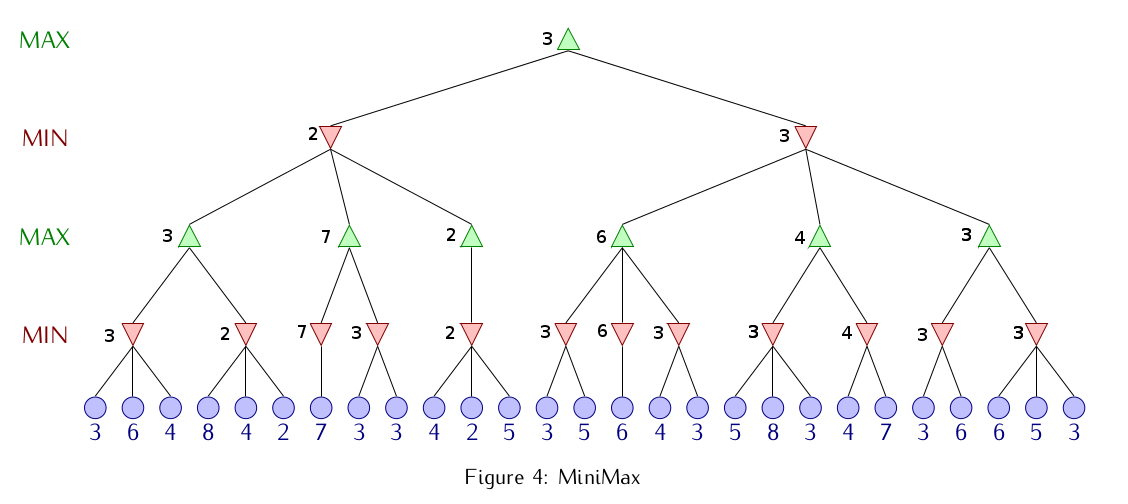
\includegraphics[scale=0.4]{minimax-fig4.png}
\item[Question 2]: Perform the Alpha-Beta algorithm on the tree in Figure 5. At each non terminal node, put the successive values of $\alpha$ and $\beta$. Cross out the arcs reaching non visited nodes. Assume a left-to-right node expansion.\\
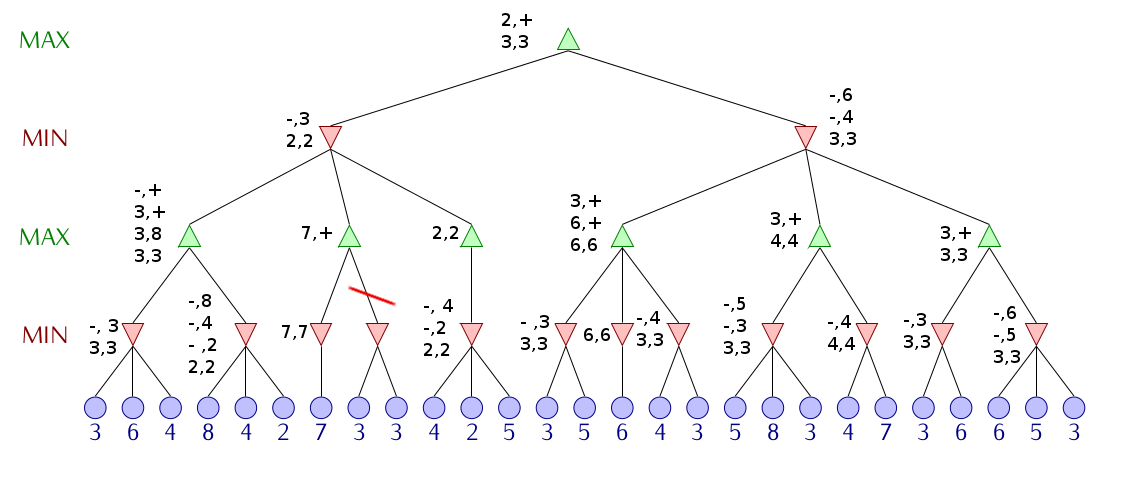
\includegraphics[scale=0.4]{minimax-fig5.png}
\item[Question 3]: Do the same, assuming a right-to-left node expansion instead (Figure 6).\\
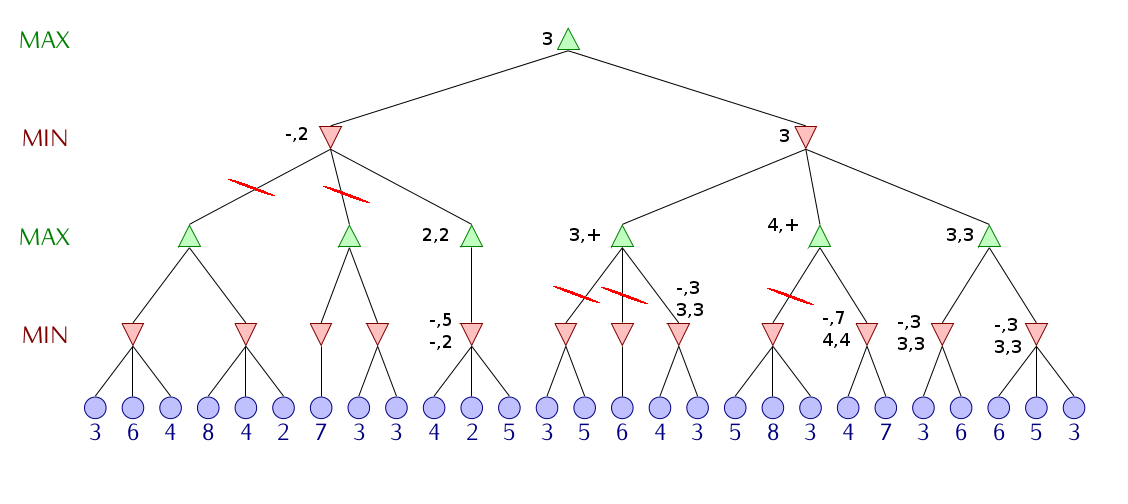
\includegraphics[scale=0.4]{minimax-fig6.png}
\item[Question 4]: Can the nodes be ordered in such a way that Alpha-Beta pruning can cut off more branches (in a left-to-right node expansion)? If no, explain why; if yes, give the new ordering and the resulting new pruning.\\
Yes. The nodes have to be ordered in an increasing way for \texttt{MIN} levels and in a decreasing way for \texttt{MAX} levels. 
\todo{Build the new tree}
\end{description}

\section{Quoridor}
\subsection{A basic Alpha-Beta agent}
\subsection{Comparison of two evaluation functions}
\begin{description}
\item[Question 4]: Launch two instances of your basic agent and make them play against each other. Use the replay options to have a look at the two first moves of both payers. What do you observe?\\
Blue player is going on the right direction. Red player is moving two same board positions. 
\item[Question 5]: Replace the basic evaluation function such that it returns directly the result of Board.get\_score instead of -1, 0 or 1. Launch again two instances of your agent and make them play against each other. Does their respective behaviour radically change? What do you observe?\\
In this situation, Red player wins. Both players went to the right direction.
\item[Question 6]: Explain why the respective behaviours of the instances of your agent changes when considering the two different evaluation function. To help you and illustrate your answer, draw and compare the search trees of depth 2 for the second move of the second player for both evaluation functions. Perform the MiniMax algorithm (not the alpha-beta) on these two trees, i.e. put a value to each node. Circle the move the root player should do.\\
\todo{Put tree here}
\end{description}

\subsection{Evaluation function}
\begin{description}
\item[Question 7]: Describe your evaluation function.\\
In our evaluation function, we compute the cost to every goal tile with a dijkstra algorithm and we take the minimal one. We compute it for both player and opponent. A special value is also evaluated if player is on a goal (to force player to go on this tile first). 
\item[Question 8]: In Alpha-Beta, the evaluation function is used to evaluate leaf nodes (when the cut-off occurs). As seen in previous questions, the pruning of Alpha-Beta depends on the order of the successors. Explain how your evaluation function could be used to (we hope) obtain more pruning with Alpha-Beta. Are there any drawbacks to your approach?\\
We could improve our evaluation function by sorting results at each depth of the tree in an increasing order for opponent playing depths and in a decreasing order for player playing depths. Even if it isn't the real value for the node, it could be a good approach to know what will probably happens in the next depths. 
\item[Question 9]: Make an agent using the successor function of the basic player (section 3.1), using your new evaluation function and cutting the tree at its root to use the evaluation function on its direct successors (you can achieve this by making cutoff always return True ). Let this agent play against another similar agent using Board.get\_score as evaluation function. Try out multiple matches and vary who plays first. How well does your evaluation function fare?\\


\end{description}
\subsection{Successors functions}
\begin{description}
\item[Question 10]: Give an upper and a lower bound on the branching factor for a search tree on the Quoridor game. Justify your answer.\\

\item[Question 11]: How does the branching factor evolve after a pawn has moved? How does the branching factor evolve after a wall has been placed? Explain.\\

\item[Question 12]: From random games (at least 100), compute the average number of possible actions at each step of the game (end the game after 100 steps). A step represents the turn of one player; i.e. if both player play one move each, two steps have been performed. Plot the results in a graph. What do you observe?\\

\item[Question 13]: Are there special moves in the game after which your branching factor changes radically? What are these moves? Explain.\\

\item[Question 14]: Are all these successors necessary to be exhaustive (think about symmetry)? Why? If not, how will you consider only the necessary states?\\

\item[Question 15]: If the number of successors is still too large, can you think of states that might be ignored, at the expense of loosing completeness?\\

\item[Question 16]: Describe your successors function.\\
Successors are computed in relation with current score (computed with get\_score). If current player is losing, it tries to place a wall around opponent. Instead of trying all possible walls on the map (which would take a large computation time), our algorithm only tries walls at four places around opponent. There are pro and cons with this strategy : in some cases, it's really good because it waits the opponent to reach the end of a board side before putting walls, so he has to make the all way back. In some cases, it's bad because it could let the opponent going further before blocking him.
\end{description}

\subsection{Cut-off function}
\begin{description}
\item[Question 17]: The cutoff method receives an argument called depth . Explain precisely what is called the depth in the minimax.py implementation.\\
The depth is a number representing anticipated actions computed. A depth of one will only look at all possible actions for the next move of the player. A depth of two will also look at all corresponding actions of the opponent after the first move. The decision will so be more meaningful. 
\item[Question 18]: Explain why it might be useful (for the Quoridor contest) to cut off the search for another reason than the depth.\\
We can stop searching in the tree if one of the player won.
\item[Question 19]: Describe your cut-off function.\\
In the cut-off function, we just check that game is not finished yet. Then we check that current depth is not deeper than maximum depth allowed. We compute depth in function of time and number of walls. Depth will increase till half time is spent than it will decrease. It starts at 3 and the maximum is 8. If current player has no more walls, depth is put to one because it only needs shortest path to a goal to play. 

\end{description}





\end{document}
